\begin{figure*}[!h]
	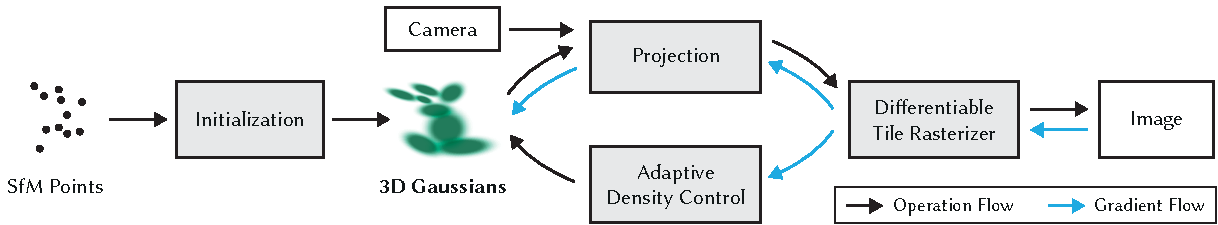
\includegraphics[width=\linewidth]{figures/overview/overview_01.pdf}
	\caption{
		Optimization starts with the sparse SfM point cloud and creates a set of 3D Gaussians. We then optimize and adaptively control the density of this set of Gaussians. During optimization we use our fast tile-based renderer, allowing competitive training times compared to SOTA fast radiance field methods. Once trained, our renderer allows real-time navigation for a wide variety of scenes.
	}
	\label{fig:overview}
\end{figure*}
\section{Overview}
The input to our method is a set of images of a static scene, together with the corresponding cameras calibrated by SfM \cite{schoenberger2016sfm} which produces a sparse point cloud as a side-effect.
From these points we create a set of 3D Gaussians %
(Sec.~\ref{sec:3d-splats}), 
defined by a position (mean), covariance matrix and opacity $\alpha$, that allows a very flexible optimization regime. This results in a reasonably compact representation of the 3D scene, in part because highly anisotropic volumetric splats can be used to represent fine structures compactly. The directional appearance component (color) of the radiance field is represented via spherical harmonics (SH), following standard practice~\cite{plenoxels,mueller2022instant}. Our algorithm proceeds to create the radiance field representation (Sec.~\ref{sec:opt-dens}) via a sequence of optimization steps of 3D Gaussian parameters, i.e., position, covariance, $\alpha$ and SH coefficients interleaved with operations for adaptive control of the Gaussian density.
The key to the efficiency of our method is our tile-based rasterizer (Sec.~\ref{sec:tile-raster}) that allows $\alpha$-blending of anisotropic splats, respecting visibility order thanks to fast sorting. Out fast rasterizer also includes a fast backward pass by tracking accumulated $\alpha$ values, without a limit on the number of Gaussians that can receive gradients. 
The overview of our method is illustrated in Fig.~\ref{fig:overview}.

